\documentclass[12pt]{article}
\usepackage[utf8]{inputenc}
\usepackage{lineno}
\usepackage{authblk}
\usepackage[margin=1in]{geometry}
\usepackage{xparse}
\usepackage{xpunctuate}
\usepackage{xspace}
\usepackage{graphicx}
\usepackage{wrapfig}
\usepackage[hidelinks]{hyperref}
\usepackage[all]{hypcap}
\usepackage{amsmath}
\usepackage{cleveref}
\usepackage{placeins}
\usepackage{flafter}
\usepackage{floatrow}
\usepackage{subcaption}
\usepackage{minted} 
\setminted[python]{breaklines}
\usepackage{caption}
\usepackage{float}
\usepackage{csvsimple}
\usepackage{booktabs}
\usepackage{siunitx}
\usepackage{natbib}

% local definitions
\newcommand{\msprime}[0]{\texttt{msprime}\xspace}
\newcommand{\tskit}[0]{\texttt{tskit}\xspace}
\newcommand{\slim}[0]{\texttt{SLiM}\xspace}
\newcommand{\pyslim}[0]{\texttt{pyslim}\xspace}
\newcommand{\stdpopsim}[0]{\texttt{stdpopsim}\xspace}
\newcommand{\allel}[0]{\texttt{scikit-allel}\xspace}
\newcommand*{\eg}{e.g.\xcomma}
\newcommand*{\ie}{i.e.\xcomma}
\newcommand{\comment}[1]{\textit{\color{green} #1}}
\newcommand{\p}[1]{\texttt{p#1}}

% syntax highlighting
\usepackage{listings}
\usepackage{xcolor}

% see listings documentation
\lstdefinelanguage{slim}{
    % Eidos language keywords from 
    % https://github.com/MesserLab/SLiM/blob/4bcc36a02aeacdc9ee808e38d62836f854246502/eidos/eidos_token.h#L90
    morekeywords=[1]{if,else,do,while,for,in,next,break,return,function},
    % SLiM callback keywords from
    % https://github.com/MesserLab/SLiM/blob/4bcc36a02aeacdc9ee808e38d62836f854246502/core/slim_eidos_block.cpp#L32
    morekeywords=[2]{first,early,late,initialize,mutationEffect,fitnessEffect,interaction,mateChoice,modifyChild,recombination,mutation,survival,reproduction},
    % Other special SLiM tokens from
    % https://github.com/MesserLab/SLiM/blob/4bcc36a02aeacdc9ee808e38d62836f854246502/QtSLiM/QtSLiMSyntaxHighlighting.cpp#L294
    morekeywords=[3]{sim,community,slimgui,
        p0,p1,p2,p3,p4,p5,p6,p7,p8,p9,p10,p11,p12,p13,p14,p15,p16,p17,p18,p19,p20,p21,p22,p23,p24,p25,
        p26,p27,p28,p29,p30,p31,p32,p33,p34,p35,p36,p37,p38,p39,p40,p41,p42,p43,p44,p45,p46,p47,p48,p49,p50,
        g0,g1,g2,g3,g4,g5,g6,g7,g8,g9,g10,g11,g12,g13,g14,g15,g16,g17,g18,g19,g20,g21,g22,g23,g24,g25,
        g26,g27,g28,g29,g30,g31,g32,g33,g34,g35,g36,g37,g38,g39,g40,g41,g42,g43,g44,g45,g46,g47,g48,g49,g50,
        m0,m1,m2,m3,m4,m5,m6,m7,m8,m9,m10,m11,m12,m13,m14,m15,m16,m17,m18,m19,m20,m21,m22,m23,m24,m25,
        m26,m27,m28,m29,m30,m31,m32,m33,m34,m35,m36,m37,m38,m39,m40,m41,m42,m43,m44,m45,m46,m47,m48,m49,m50,
        s0,s1,s2,s3,s4,s5,s6,s7,s8,s9,s10,s11,s12,s13,s14,s15,s16,s17,s18,s19,s20,s21,s22,s23,s24,s25,
        s26,s27,s28,s29,s30,s31,s32,s33,s34,s35,s36,s37,s38,s39,s40,s41,s42,s43,s44,s45,s46,s47,s48,s49,s50,
        i0,i1,i2,i3,i4,i5,i6,i7,i8,i9,i10,i11,i12,i13,i14,i15,i16,i17,i18,i19,i20,i21,i22,i23,i24,i25,
        i26,i27,i28,i29,i30,i31,i32,i33,i34,i35,i36,i37,i38,i39,i40,i41,i42,i43,i44,i45,i46,i47,i48,i49,i50},
    sensitive=true,
    morecomment=[l]{//},
    morestring=[b]",
}
% colors from 
% https://github.com/MesserLab/SLiM/blob/4bcc36a02aeacdc9ee808e38d62836f854246502/QtSLiM/QtSLiMSyntaxHighlighting.cpp#L139
% numberLiteralFormat.setForeground(inDarkMode ? QColor(115, 145, 255) : QColor(28, 0, 207));
% stringLiteralFormat.setForeground(inDarkMode ? QColor(220, 98, 90) : QColor(196, 26, 22));
% commentFormat.setForeground(inDarkMode ? QColor(90, 210, 90) : QColor(0, 116, 0));
% identifierFormat.setForeground(inDarkMode ? QColor(70, 205, 216) : QColor(63, 110, 116));
% keywordFormat.setForeground(inDarkMode ? QColor(220, 83, 185) : QColor(170, 13, 145));
\definecolor{slimstring}{RGB}{196,26,22}
\definecolor{slimcomment}{RGB}{0,116,0}
\definecolor{slimidentifier}{RGB}{63,110,116}
\definecolor{slimkeyword}{RGB}{170,13,145}
\definecolor{slimstage}{RGB}{0,0,0}
\definecolor{codegray}{RGB}{128,128,128}
% Light beige background for SLiM code (different from Python's gray background)
\definecolor{backcolour}{rgb}{0.95,0.95,0.92}
\lstdefinestyle{slimstyle}{
    language=slim,
    backgroundcolor=\color{backcolour},
    commentstyle=\color{slimcomment},
    keywordstyle=[1]\color{slimkeyword},
    keywordstyle=[2]\color{slimstage},
    keywordstyle=[3]\color{slimidentifier},
    numberstyle=\tiny\color{codegray},
    stringstyle=\color{slimstring},
    basicstyle=\ttfamily\small,
    escapeinside={*@}{@*},
    breakatwhitespace=false,         
    breaklines=true,                 
    captionpos=b,                    
    keepspaces=true,                 
    numbers=left,                    
    numbersep=2pt,                  
    showspaces=false,                
    showstringspaces=false,
    showtabs=false,                  
    tabsize=2
}
\lstset{style=slimstyle}

% Fix for quote encoding issues
% https://tex.stackexchange.com/questions/736299/latex-error-command-textquotedbl-unavailable-in-encoding-ot1
\lstset{upquote=true,basicstyle=\fontencoding{T1}\selectfont}

\definecolor{bg}{rgb}{0.95,0.95,0.98}
\newminted[pycon]{pycon}{bgcolor=bg, linenos=true, tabsize=4}

%\linenumbers

\begin{document}

\title{Bridging forward-in-time and coalescent simulations using pyslim}
\author[1]{Shyamalika Gopalan}
\author[2,3]{Murillo F. Rodrigues}
\author[3,4]{Peter L. Ralph}
%\author[5]{Ben Haller}

\affil[1]{Department of Genetics and Biochemistry and Center for Human Genetics, Clemson University}
\affil[2]{Division of Genetics, Oregon National Primate Center, Oregon Health \& Science University}
\affil[3]{Department of Biology and Institute of Ecology and Evolution, University of Oregon}
\affil[4]{Department of Mathematics, University of Oregon}
%\affil[5]{Department of Computational Biology, Cornell University}

\maketitle

\abstract{
    Ancestral Recombination Graphs (ARGs)
    provide an expressive and compact way to represent genetic variation data generated by simulations
    embedded within its genealogical history,
    and can dramatically speed up simulations.
    The fact that the ARG records genealogical as well as genomic information
    opens up the possibility for a number of new analysis and simulation techniques.
    Here, we aim to introduce the reader to this deep source of information
    as produced by the forwards simulator SLiM.
    SLiM records the ARG using the \emph{tree sequence} format,
    which can be manipulated using the \tskit and \pyslim python packages.
    We first describe the information that SLiM records in the tree sequence,
    then provide several examples that use the tree sequence as a format
    to losslessly pass population states between simulators:
    \emph{recapitation} of a fowards simulation with coalescent simulation;
    initiation of a forwards simulation using the results of a coalescent simulation;
    and parallelization of simulations, first across branches of a phylogenetic tree
    and then between individuals in a host-parasite simulation.
}
\date{}


\section*{Introduction}
% The importance of simulations in popgen and flavors of simulations
Simulations have become an invaluable tool in population genetics over the past six decades,
allowing researchers to model increasingly complex evolutionary scenarios.
%because of the difficulty in obtaining analytical solutions to complex evolutionary scenarios.
A robust research community has grown around developing computational methods for conducting these
simuations, as well as for representing and analyzing the data that they produce.
Indeed, in prior chapters, two of the most widely used population genetic simulation tools were presented: \slim \citep{haller_slim_2023} and \msprime \citep{baumdicker_efficient_2022}.
% refer to other chapters here?

In this chapter, we present \pyslim, a Python package that facilitates \emph{hybrid simulations},
which combine key features of the two main methods of population genetic simulation.
These two methods differ primarily in the direction of the simulation
process -- either forward- or backward-in-time. 
The coalescent process models the ancestry of sampled genomes
backward-in-time until they coalesce into their most common recent ancestor. % (MRCA).
This approach is extremely efficient because it only has to simulates the ancestors that directly contributed to the sampled genomes,
thus avoiding the need to represent large swathes of the population tree. 
The downside of this approach is its strict assumptions(\eg neutrality), 
which limit applicability to more complex evolutionary questions.
On the other hand, forward-in-time simulations start with the ancestral genomes and apply evolutionary rules (\eg mutation, recombination, selection) over generations.
This affords forward-in-time simulations much more flexibilty in modelling non-neutral scenarios, 
but at a high computational cost.
% refer to msprime and SLiM chapters explicitly here?
% The pyslim package and overview of the chapter

Hybrid simulations have recently emerged as a strategy for leveraging the benefits of both forward-in-time and coalescent methods
to efficiently model highly complex evolutionary scenarios.
Most forward-in-time simulations conducted using \slim, for example, are later modified using the coalescent process to ensure the coalescence of the individuals in the first generation, a process known as \emph{recapitation} which will be discussed in more detail later in this chapter.
\stdpopsim, a Python package that stores a large number of published population genetic models,
uses a hybrid approach to ensure the coalescence of the individuals in the first generation of the forward-in-time simulation \citep{adrion_community-maintained_2020,elise_expanding_nodate,gower_accessible_2025}.
In complex spatial forward-in-time simulations, a coalescent component is almost always present,
and it can reduce significantly the computational burden of these simulations \citep{battey_space_2020,petr_slendr_2023}.
A hybrid simulation approach made possible to perform whole-chromosome simulations of the entire great apes history, a clade with over 10 million years of history in \citet{rodrigues_shared_2024}.

% something here to motivate the pathogen evolution scenario we present?

A key innovation that has enabled the rise of hybrid simulations is the concept of the Ancestral Recombination Graph (ARG), reviewed in \citet{wong_general_2024}.
Compared to genotype data encoding, the ARG represents a much richer source of information about the processes that gave rise to a given set of genomes \citep{kelleher_efficient_2016}.
Importantly, popular versions of both coalescent (\eg msprime) and forward-in-time (\eg SLiM) simulation software share a common format for
encoding the ARG: the ``tree sequence'' data structure \citep{baumdicker_efficient_2022, haller_tree-sequence_2019}.
This has made it possible for simulations to be started using either forward- or backward-in-time
methods and then be continued using the alternative approach, thereby resulting in a 'hybrid' simulation.

Here, we will review how \slim, a popular forward-in-tim simulation software, uses the tree sequence before describing
the main uses of \pyslim in conducting hybrid simulations, specifically:
(i) recapitation, the process of simulating the history of uncoalesed first-generation individuals,
(ii) generation of initial diversity using the coalescent process for forward-in-time simulations,
(iii) parallelization of multi-population simulations.
Finally, to illustrate the realism that can be achieved with a hybrid approach, we present a vignette of an organism evolving under a complex life history.
Some of the text in this chapter has been adapted from \pyslim's documentation.
(\url{https://tskit.dev/pyslim/docs/latest}).

%%%%%%%%%%%%%%%%%%%%%
\section{Tree sequences and SLiM}
As described in \citet{wong_general_2024}, the term ``ancestral recombination graph'' (ARG)
represents the paths of genealogical inheritance that have produced a given set of genomes,
and the \emph{tree sequence} format of \tskit provides a general-purpose way to store ARGs.
For this reason, we mostly use the term ``tree sequence'' in this chapter even where ``ARG'
would be equally accurate, as well as other terminology associated with \slim and \tskit \citet{kelleher_efficient_2016,ralph_efficiently_2020,wong_general_2024}.

As SLiM proceeds with simulating genomes evolving forward-in-time, it tracks how all the genomes are
related to each other and returns the result as an ARG in tree sequence format. First, we describe
exactly \emph{what} information is recorded, \emph{how} it is recorded, and how to access it.

\paragraph{Terminology:}
Each \textit{node} of a tree sequence represents a single (haploid) genome;
inheritance relationships between these are recorded as \textit{edges},
and genetic variation is represented by \textit{mutations} at associated \textit{sites}.
A particular tree sequence describes the entire genealogy of a set of ``focal'' nodes called
\textit{sample nodes}, or simply \textit{samples}, over the simulated time period.
Many \tskit operations act on these sample nodes by default.
The samples are those genomes for which we have complete genetic ancestry information; for the other 'non-sample'
nodes in the tree sequence, which are required to describe that ancestry, we might only have partial information
('Who is and isn't in the tree sequence' below gives more detail about sample nodes).
By default, SLiM simulates diploid organisms, where each \textit{individual} is represented by two nodes.

Since SLiM is a forwards simulator, it records time (in units called ``ticks'')
since the start of the simulation, with 0 corresponding to the earliest time point.
We call this \textit{SLiM time}.
However, in many cases, a more natural point of reference might be in relation to the samples, with
time in the tree sequence measured in units of \textit{time ago}. This is the same way that time
is represented in coalescent or backward-in-time approaches, with the 0th time point corresponding
to the end of the simulation rather than the beginning. This dual representation of time is important
to consider when thinking about hybrid simulations, as we will see later in the chapter.

\begin{figure}
\centering
    \subcaptionbox{All relationships.}{\vspace{0em}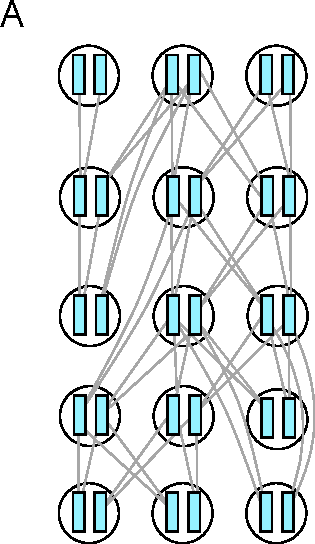
\includegraphics[width=0.3\textwidth]{figures/pedigree0.pdf}\hspace{0em}} % MFR: I added these spaces because for some weird reason Inkscape keeps crashing when I try to edit the original svgs
    \hfill
    \subcaptionbox{Those relationships left at the end of the simulation.}{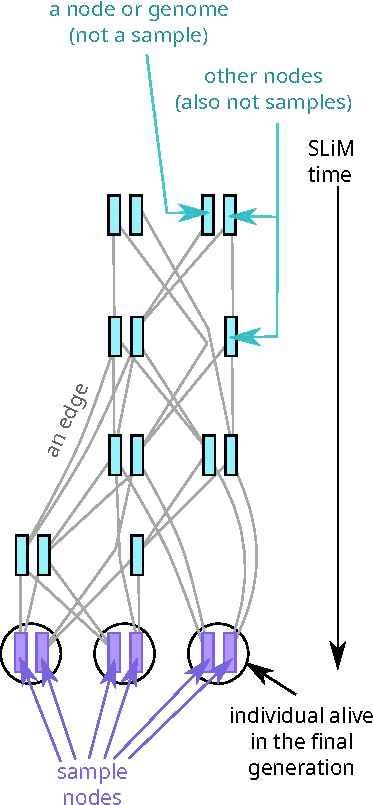
\includegraphics[width=0.3\textwidth]{figures/pedigree2.pdf}}
    \hfill
    \subcaptionbox{Additional individuals may be ``remembered'' (purple)
        or ``retained'' (dotted).}{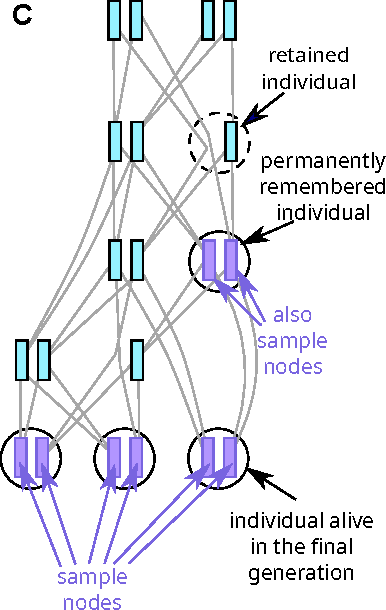
\includegraphics[width=0.3\textwidth]{figures/pedigree_remember.pdf}}
\caption{
    The resulting genetic relationships between individuals in a small simulation
    (three diploids over five generations).
}
\label{fig:indivs}
\end{figure}

\paragraph{Who is and isn't in the tree sequence:}
Suppose we have run a very small simulation with SLiM. The genetic relationships among each of the
diploid individuals who were alive over the course of the simulation might
look something like Figure~\ref{fig:indivs}A. Since individuals (circles) are diploid, each contains
two genomes or nodes (shaded rectangles).
The edges of the tree sequence record which specific parts of the genome are inherited,
so the relationships recorded in the tree sequence are between the nodes and not the individuals directly.

In many cases, samples nodes will be drawn from individuals that are still alive in the final generation
of the simulation. This renders large portions of the tree sequence irrelevant, as they
correspond to lineages that died out at some earlier point in the simulation (but see section below on
'Historical Individuals' about how to model ancient samples in a SLiM/tree sequence framework). To avoid having to
store this large quantity of unnecessary information, SLiM periodically \textit{simplifies} the tree sequence
as the simulation goes along. By default, simplification will only keep the portions of the
genetic genealogy that are required to represent the history of the current nodes
\citep{kelleher}. Additionally, it defaults to removing any node that is not a genetic
\textit{most recent common ancestor} (MRCA) of at least two daughter nodes. This removes historical
nodes that are only ``on the line to'' a sample, but do not represent a branching point
(\ie coalescent event) on the tree. These 'unary nodes' can be retained within SLiM, and they are
sometimes necessary for tree sequence merging, as we discuss below.

As a result of the simplification process, the output tree sequence will look something like Figure~\ref{fig:indivs}B.
To be precise, edges correspond to genomic \emph{segments} with defined start and end positions,
but we do not attempt to depict that complexity here. Instead, this figure can be thought of as representing a simulation
with no recombination, so entire nodes, rather than genomic segments, are being inherited.

Individuals who are alive at the end of the simulation automatically have their nodes marked as
\textit{samples}. All other historical (\ie dead) individuals (depicted as circles) have vanished,\
although some of their nodes remain. As discussed previously, these nodes have only been retained because they are required to
accurately represent the ancestry of one or more sample nodes and/or the relationships among sample nodes.
Put simply, simplification removes any nodes, along with any associated edges,
that have not made a genetic contribution to the sample set of nodes.

%%%%%%%% %%%%%%%%%%%%%%
\section*{Historical individuals}
By default, only the nodes associated with individuals alive in the final generation are part of the 'sample' set.
However, there are many cases where we might want to retain the complete ancestry, and other metadata, for
historical nodes. For example, we might want to model the relationship between a modern population and
one particular individual from the past. Or, if we are conducting simulations in parallel that share 
a common ancestry, we may need to retain certain nodes that are critical for linking distinct
tree sequences back together.
In order to accomplish this, we can choose to ``remember'' key individuals during the course of the simulation,
using the SLiM function \verb|treeSeqRememberIndividuals()|.

\paragraph{Permanently remembering individuals}
By default, a call to \\ 
\verb|treeSeqRememberIndividuals()| will permanently remember one or more individuals,
the simulated equivalent of ancient DNA dug out of permafrost.
This means that any tree sequence subsequently recorded will always contain this individual,
its nodes (now marked as samples), and its full ancestry.
The result of remembering an individual in the introductory example is pictured
in Figure~\ref{fig:indivs}C.
This is also useful to, for instance, access allele frequencies and spatial locations of individuals
at a particular time in the past.

\paragraph{Retaining individuals}
Alternatively, you may want to only retain historical individuals as long as their nodes are still
relevant to reconstructing the genetic ancestry of the sample nodes.
This retains information that is specific to individuals as opposed to their nodes,
such as their two parents (in diploid simulations) and their location (in spatial simulations), that would otherwise be 'cleaned up' during simplification.
This is less burdensome than remembering everyone alive, as individuals can still be removed once their
nodes (which are not marked as samples) are no longer ancestral.
You can \emph{retain} individuals in this way by using
\verb|treeSeqRememberIndividuals(..., permanent=F)|.
Since a retained individual’s nodes are not considered samples,
they are subject to the standard removal 'rules' of simplification.
It is therefore possible to end up with an individual containing only one genome, as shown in the diagram.
However, as soon as both nodes of a retained individual have been lost,
the individual and any information associated with it is deleted too.

As previously discussed, simplification will, by default, only keep nodes if they are a coalescent point
(\ie they are a MRCA or branch point) somewhere along the genome.
This can be changed by initialising tree sequence recording in SLiM using
\verb|treeSeqInitialize(retainCoalescentOnly=F)|.
SLiM will then preserve all retained individuals while they remain in the genealogy of present-day individuals,
even if their nodes are not coalescent points in the tree.
If you later decide to reduce the number
of samples in the tree sequence, you can do so using the tskit function simplify(),
which mirrors SLiM's version of the same procedure.
In this case, individuals that are 'retained' rather than 'remembered' will be kept only
if they are still MRCAs in the ancestry of the selected samples.
To preserve them even if their nodes are not coalescent points,
you can specify \verb|ts.simplify(selected_samples, keep_unary_in_individuals=True)|.

%%%%%%%%%%%%%%%%%%%%%%%
\section{Recapitation: tying up loose ends} %% "Streamlining the burn-in, two ways"

\begin{figure}
\centering
    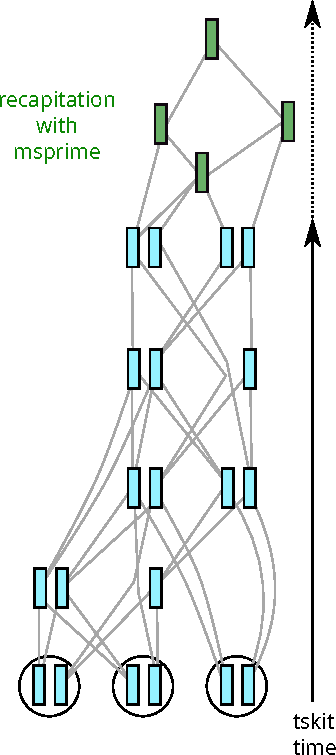
\includegraphics[width=0.2\textwidth]{figures/pedigree_recapitate.pdf}
    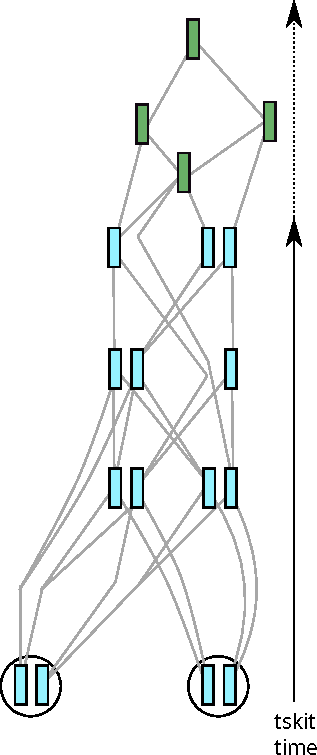
\includegraphics[width=0.2\textwidth]{figures/pedigree_simplify.pdf}
\caption{
    \textbf{(A)} Recapitation adds the green nodes 
    to the simulation of Figure~\ref{fig:indivs} by coalescent simulation.
    \textbf{(B)} The result of \emph{simplifying} the tree sequence in (A)
    down to the four sample nodes shown.
}
\label{fig:recap_simp}
\end{figure}

By default, a \slim simulation begins with all individuals being identical, and genetic diversity
builds up over time as new mutations occur. However, in many cases, starting with a clonal population
is undesirable and can have long-lasting effects on patterns of diversity in the samples. One way to overcome
this is to include a long ``burn-in'' period in the forward simulation to reach an 'equilibrium' level of genetic diversity.
However, this period generally needs to be quite long (on the order of 5--15 times the effective population size, in generations),
which can be prohibitive for computationally expensive forward-in-time simulations.
An efficient alternative is to ``seed'' the simulation with genetic diversity generated by a coalescent simulation, i.e. conduct a hybrid simulation.
There are two main ways to do this, which we refer to as ``recapitation'' and ``generating initial diversity'', respectively.
These approaches have distinct purposes, but the main difference between them is when
this coalescent step is run, relative to the forward-in-time portion of the simulation. We will discuss these approaches in the following two sections.

Recapitation is performed to the tree sequence that is generated after a SLiM simulation has already been run.
This may be suitable when the SLiM step does not require the ancestral genotypes for anything, such as determining individual fitness,
and all that is needed are realistic genealogical relationships. Functionally, recapitation conducts a coalescent simulation
starting with the first-generation ancestral nodes (SLiM time 0) that have not yet coalesced.
This is discussed in more detail in \citet{kelleher} and \citet{slim_manual}.

Figure~\ref{fig:recap_simp}A illustrates this process: imagine that, at some sites, one or more samples do not share
a common ancestor within the SLiM simulated portion of history (shown in blue).
Recapitation starts at the \textit{top} of the genealogies and moves backwards in time
to fill in a genealogical history for all the samples.
In Figure~\ref{fig:recap_simp}B?, the green chromosomes are new ancestral nodes that have been added to the tree sequence.
As previously mentioned, the effect of omitting this step would be to model a genetically homogeneous initial population;
our simulation would have less genetic variation than it ``should'' have, since the all the variation
contributed by the 'green' portion of the tree would be omitted.

It is important to consider how time is conceptualized in this hybrid simulation. In forward simulation (i.e. SLiM) time,
the first-generation ancestors at the top of the blue portion of the genealogy are ``born'' at time 0. When we recapitate the genealogy,
nodes in the green portion of the genealogy will necessarily be born in negative SLiM time since they arise before the events of the
forward-in-time portion of the simulation. In coalescent time, the age of the recapitated nodes simply increases relative to the final generation
(i.e. the set of nodes at the \textit{bottom} of the blue genealogy). %% could be explained more clearly, i think (SSG)

Recapitation within a single randomly-mating population of a given size
can be achieved with a simple call to \verb|pyslim.recapitate(ts, ancestral_size=N)|
Since pyslim.recapitate is a wrapper around
msprime.sim\_ancestry, we could recapitate our tree with any model that can be represented by \msprime code
\citep{baumdicker}. For instance, it is possible to recapitate a SLiM-generated tree sequence with a fluctuating population size
or non-uniform genetic map by simply passing in the relevant arguments.

Setting up a demographic model in \msprime that is consistent and compatible with a particular SLiM simulation requires
understanding some of the finer details of each of these software packages, so here we will present a concrete example.
Consider the following two-population model in SLiM:

We'll demonstrate recapitation with a two-population model,
since setting up an \msprime demographic model that is consistent with the SLiM simulation
requires understanding some of the details.
Recapitation happens by passing the tree sequence to the
\texttt{initial\_state} argument of \texttt{msprime.sim\_ancestry},
along with a demographic model.
The root of each uncoalesced lineage in the tree sequence is a node
that exists at a particular time and in a particular population;
these two things situate the linear within the demographic model,
so \msprime can continue following the lineages back through time.
Suppose that we've used \slim to simulate two populations, \ie with the following block:
\begin{lstlisting}{language=slim}
% add init stuff
% what is K? does K need to match init_size below?
\begin{minted}[fontsize=\small, linenos, bgcolor=gray!10]{slim}
>>>>>>> origin/main
1 early() {
   sim.addSubpop("p1", K);
   sim.addSubpop("p2", K);
}
%% add write out ts
\end{lstlisting}
\end{minted}
\comment{TODO provide link to or name of full slim recipe}

If the resulting tree sequence is stored in the file \texttt{recap_example.trees},
then examining the populations using the shell, we see:
%\begin{lstlisting}{language=bash}
%> tskit populations recap_example.trees
%id	metadata
%0	None
%1	{'name': 'p1', 'slim_id': 1}
%2	{'name': 'p2', 'slim_id': 2}
%\end{lstlisting}
%%% SSG - my output looks a little different, maybe because i'm running SLiM 5?
\begin{lstlisting}{language=bash}
> tskit populations recap_example.trees
id	metadata
0	None
1	{'migration_records': [], 'name': 'p1', 'sex_ratio': 0.0, 'slim_id': 1}
2	{'migration_records': [], 'name': 'p2', 'sex_ratio': 0.0, 'slim_id': 2}
\end{lstlisting}

There are \emph{three} populations, but the first one is unused, because \slim stores population \texttt{pX} as population \texttt{X}.
To be compatible with this tree sequence, the \msprime demographic model will need to include three populations as well.
However the first population will remain unused unless we specify it as an ancestral source for
one of the other two populations during the coalescent phase of the simulation. Note that we could have avoided having this
'dummy' population if we had named our two populations 'p0' and 'p1' within the SLiM script. Similarly, if we would have started
numbering our populations from 'p3', we would end up with a total of three 'dummy' populations in our tree sequence.

Regardless of the population numbering scheme used, \msprime provides a built-in method of seamlessly generating a
compatible demography given a particular starting tree sequence file. The following code reads the tree sequence ``ts''
and creates a basic demography from the information contained therein: 
\begin{lstlisting}{language=py}
%% read recap_example.trees as ts?
demography = msprime.Demography.from_tree_sequence(ts, initial_size=100)
\end{lstlisting}

The resulting demography specifies 3 populations with an effective size of 100 individuals each. Not that the initial_size
does not have to match what we specified in our SLiM simulation, because it specifies the size of the generation
immediately preceding the SLiM phase. We could theoretically try to recapitate our tree sequence with this
demography, but if we did so, \msprime would run forever. This is because we have not allowed for any way for
lineages from p1 to coalesce with lineages in p2, or vice versa. Therefore, the coalescent process will never be able to conclude.

To remedy this, we need to provide a migration path that allows lineages from different populations to coalesce.
Let us specify one-directional migration from \p1 to \p2, such that lineages in \p2 move into \p1 as we move backwards in time
starting 100 generations before the start of the SLiM simulation. Note here that 'time' here must be specified in terms of the coalescent process:
\begin{lstlisting}{language=py}
demography.add_migration_rate_change(
    time=ts.metadata['SLiM']['tick'] + 100,
    rate=0.1, source="p2", dest="p1",
)
rts = pyslim.recapitate(ts, demography=demography,
            recombination_rate=1e-8)
\end{minted}

The \pyslim function 'recapitate' passes the tree sequence 'ts' to the
\texttt{initial\_state} argument of \texttt{msprime.sim\_ancestry},
along with the demographic model that we specified.
The root of each uncoalesced lineage in this tree sequence is a node
that exists at a particular time and in a particular population;
these two things situate the lineage within the demographic model,
allowing \msprime to continue following the lineages back through time.

\section{Generating initial diversity} % better name for this process? this doesn't have the same ring as 'recapitation'

Another way to ``seed'' a forward-in-time simulation with a baseline level of genetic diversity
is to run a neutral coalescent process first to generate a starting tree sequence. This tree sequence
can then be loaded into \slim where the main simulation process can proceed as normal. This
approach is useful when simulating selection on standing variation in a large population, where
a purely forward-in-time burn-in period would be very costly in terms of time and computational resources.
Because the genetic variation needs to exist in the population at the start of the simulation, adding
it on after the fact via recapitation, as discussed in the previous section, is not an option. While running
a neutral coalescent burn-in is not exactly the same as a running a forward-in-time burn-in with selection,
this can be an adequate approximation in most cases. %citations to this effect?

Imagine that we want to perform a lab experiment in which we take high-diversity
organisms from the wild and subject them to selection for a few dozen generations.
Although genetic diversity in the wild population is most likely not neutral,
we do not know precisely what the selection coefficients are for each variant.
However, the key attribute of reality we would like to approximate is the joint distribution of
allele frequencies and effect sizes. Broadly speaking, we can expect an overall negative correlation
between effect size and allele frequency for a trait under stabilizing selection; i.e. the larger
the effect of an allele, the lower its frequency in the population.
On the other hand, there would be no relationship between allele frequencies and effect sizes
if the trait we are selecting on in the lab is not under strong selection in the wild.
For our example, we will assume the latter: that the trait we are selecting for in the lab was
not under stabilizing selection in the wild. To implement this, we will:
(1) run a coalescent simulation with msprime;
(2) ``annotate'' the resulting tree sequence with \slim metadata;
(3) add \slim mutations with msprime
        and edit the mutation metadata to assign selection coefficients; and finally
(4) run the \slim portion of the simulation.

\subsection*{Annotating tree sequence with SLiM metadata}

Suppose we run the following coalescent simulation in \msprime to produce the tree sequence \verb|ts|:

\begin{listing}[H]
  demog_model = msprime.Demography()
  demog_model.add_population(initial_size=1_000)
  ts = msprime.sim_ancestry(
          samples=1_000,
          demography=demog_model,
          random_seed=5,
          recombination_rate=1e-8,
          sequence_length = 90_000_000)
\end{listing}

This tree sequence is a complete record of the genealogical information relating specific individuals
and nodes, but is missing other information that  SLiM requires to read it in and use it as an initial state.
We can use \pyslim to easily add this information to our tree sequence using the ``annotate'' function.
In fact, this function goes beyond simply annotating to ensure that the \msprime-generated tree sequence
is compatible with SLiM by also having the user define the model type (Wright-Fisher or non-Wright-Fisher)
and specify how coalescent- and SLiM-time\ should be aligned.

\begin{listing}[H]
  \begin{minted}[fontsize=\small, linenos, bgcolor=gray!10]{python}
    ats = pyslim.annotate(ts, model_type="WF", tick=1, stage="late")
  \end{minted}
\end{listing}

This code fills in the default values for every element of the tree sequence that requires it. 
In this case, that includes all individuals, all nodes that exist within living individuals, and all
populations referenced by nodes. We can see exactly what these defaults
are for any given component of the tree sequence by using 'default_slim_metadata':

\begin{listing}[H]
  \begin{minted}[fontsize=\small, linenos, bgcolor=gray!10]{python}
    pyslim.default_slim_metadata("individual")
    pyslim.default_slim_metadata("node")
    pyslim.default_slim_metadata("population")
  \end{minted}
\end{listing}

We can see that pyslim.annotate will designate all individuals as hermaphroditic (individual 'sex' is -1) and
all chromosomes as autosomal (node 'genome_type' is 0). It is possible to change these values in order to,
for example, define sexes. Below, we show how to do this specifically for mutations, but other modifications
can be done in a similar manner.

\subsection*{Adding mutations with SLiM metadata}-

The next step in this process is the generate the initial genetic diversity that natural selection will act on
in the forward-in-time phase of our hybrid simulation. Let us assume an overall rate of 3e-8 new
mutations per base pair per generation. Further, let us assume that 99\% of all new mutations
are neutral. If we were doing this simulation entirely within a forward-in-time framework with a long
burn-in, we could have achieved this outcome using the following \slim code:

\begin{lstlisting}{language=slim}
        initializeMutationType("m2", 0.5, "f", 0.001);
        initializeMutationRate(3e-10);
\end{lstlisting}

This code defines a mutation type \verb|m2| that has a dominance coefficient of 0.5 and a fixed selection
coefficient of 0.001 (the latter can be made more flexible, e.g. drawn from a distribution - see \slim manual).
Notice, too, that we have set these non-neutral mutations to arise at a rate of 3e-10 per base per generation,
or 1\% of our desired overall mutation rate of 3e-8. To approximate this result using \msprime, we must first
use the function \verb|SLiMMutationModel| to apply some mutations to the existing tree sequence:

\begin{listing}[H]
  \begin{minted}[fontsize=\small, linenos, bgcolor=gray!10]{python}
    mut_model = msprime.SLiMMutationModel(type=2)
    mts = msprime.sim_mutations(ats, rate=3e-10, model=mut_model)
  \end{minted}
\end{listing}

The \verb|type=2| argument denotes that the mutations will be of type ``m2'' in SLiM, which will also
need to be explicitly initialized in the forward-in-time phase of the simulation (see below).
By default, these mutations are assigned a selection coefficient of 0, which is accurate since they
all arose in the neutrally-evolving portion of the tree. However, since we want selection to come into
effect for the SLiM phase, we will need to update the selection coefficients of these variants to reflect that.
Tree sequences are, for efficiency purposes, not directly modifiable. Therefore, to update any aspect of
a particular tree sequence we need to instead copy its underlying tables, modify the ones we need to,
and then re-generate the tree sequence. Below, we show how to apply this procedure to modify the
selection coefficient for all existing mutations:

\begin{listing}[H]
  \begin{minted}[fontsize=\small, linenos, bgcolor=gray!10]{python}
    tables = mts.dump_tables()
    tables.mutations.clear()
    for m in mts.mutations():
      md_list = m.metadata["mutation_list"]
      for md in md_list:
        md["selection_coeff"] = 0.001
        tables.mutations.append(m.replace(metadata={"mutation_list": md_list}))

    sts = tables.tree_sequence()
  \end{minted}
\end{listing}

To reiterate, this code first copied all the tables that describe the tree sequence \verb|mts|, cleared all the
information in the mutations table, and then added each existing mutation back with a new selection
coefficient. Finally, it generated a new tree sequence with this new mutation table. If we print a single
mutation from the 'before' and 'after' tree sequences, we can see the change:

\begin{listing}[H]
  \begin{minted}[fontsize=\small, linenos, bgcolor=gray!10]{python}
  mts.mutation(0)
  sts.mutation(0)
  \end{minted}
\end{listing}

As we intended, every piece of information about this mutation is the same except the selection coefficient. The resulting tree
sequence can now be read into \slim in order to proceed with the forward-in-time phase of our coalescent simulation.

Before we proceed to that step, however, we need to discuss how mutations are represented in both \slim and \tskit, as this has
implications for hybrid simulations. In \tskit, mutations are associated with sites, elements that represent a specific
position in the genome. Mutations occur at sites and have additional properties such as type (e.g. m2), time (when it arose),
node (the specific genome it arose in), and selection coefficient. If a mutation occurs at a site where a mutation already exists,
the most recent mutation will replace it. This differs from \slim, which, by default, allows recurrent mutations at the same genomic
position to 'stack' on top of each other. However, even though mutations technically do not stack in \tskit, the tree sequence
format stores the information required to represent recurrent mutation events in the data associated with each mutation.
Consider the following example of a 'double hit' mutation:

\begin{listing}[H]
    \begin{minted}[fontsize=\small, linenos, bgcolor=gray!10]{python}
Mutation(id=295, site=180, node=43931, derived_state='193,194',
    parent=294, time=8.74,
    metadata={'mutation_list': [
        {'mutation_type': 2, 'selection_coeff': 0.001, 'subpopulation': -1, 'slim_time': -559, 'nucleotide': -1},
        {'mutation_type': 2, 'selection_coeff': 0.001, 'subpopulation': -1, 'slim_time': -7, 'nucleotide': -1}
    ]})
    \end{minted}
\end{listing}

This mutation occurred
above node 43931 at a position on the genome we could obtain by looking at site 180.
Genomes that inherit this mutation carry at this site two \slim mutations with IDs 193 and 194;
these mutations are labeled with \slim time -559 and -7 generations, respectively.
Since the first of the two occurred longer ago (a larger negative \slim time),
we can infer that the mutation with \slim ID 194 occurred on the background
of the mutation with \slim ID 193.
% We can confirm this by looking at the ``parent'' mutation whose ID is 294,
% and has derived state simply 193.
Sharp-eyed readers will note that the ``time'' of the mutation given by the tree sequence
(8.74 generations ago) does not match the ``\slim time'' recorded in metadata
(-7 generations in the future);
in general this conversion is ``rounded and maybe off by one, depending on the model type''.
For a detailed discussion of conversion between time in the tree sequence
and time in the SLiM model, see the pyslim documentation.
>>>>>>> origin/main

There are two parts of this record that give away the fact that this was a recurrent mutation. First, the recorded 'derived_state' is
actually two distinct states separated by a comma. Second, the 'mutation_list' element of the mutation's metadata lists two distinct
events, one occurring 559 ticks ago and one occurring 7 ticks ago. Technically, this mutation corresponds only to the most recent
mutational event, but \tskit keeps a detailed record of what happened prior to this. This allows \slim to reconstruct these events in order
to apply the appropriate stacking policy if this tree sequence is used as an initial state for a forward-in-time simulation. So, for example,
we can infer that a mutation occurred at this site at slim_time -559 producing a derived state of 193, and then another mutation
occurred at the same site at slim_time -7 producing a derived state of 194. If another mutation occurred in a different node carrying
the same initial mutation, it would be recorded as a separate mutation in the mutation tables. Therefore, one can think of each mutation
record as representing a distinct lineage of mutations all occurring at a particular genomic location. This is why, when modifying
the selection coefficients of each mutation earlier in this section, we had to have two nested loops - one iterated over each entry of the
mutation table while the second updated each element of the associated 'mutation_list'.

Sharp-eyed readers will note that the ``time'' of the mutation given by the tree sequence (8.74 generations ago) does not exactly
correspond to the ``\slim time'' recorded in metadata (-7 generations in the future); in general this conversion is ``rounded and sometimes
off by one, depending on the model type''. For a detailed discussion of how time is converted between the tree sequence and the SLiM
model, see the pyslim documentation.

\subsection*{Loading into SLiM}

We can finally move onto the forward-in-time component of our hybrid simulation using \slim. First, we will load in the tree sequence we just
generated using \msprime and modified using \pyslim and \tskit from a file called 'init.trees'. We need to ensure that everything matches
across this tree sequence and the SLiM model that we are setting up. Specifically, the genome length defined in SLiM must be equal to the
result of the 'sequence_length' property of the tree sequence to be loaded and used as an initial state. We will also define an \verb|m2|
mutation type to match the process we used to generate mutations for the tree sequence. Additionally, we will define a placeholder mutation
type \verb|m1| for neutral mutations, to be added later. The population size(s) are automatically inferred by \slim from the tree sequence,
but we will make a point to ``Remember'' all the individuals who are alive at the start of the simulation to facilitate downstream analysis.

\begin{lstlisting}[language=slim]
initialize()
{
    initializeSLiMModelType("WF");
    initializeTreeSeq();
    initializeMutationRate(3e-10);
    initializeMutationType("m1", 0.5, "f", 0.0);
    initializeMutationType("m2", 0.5, "s", 0.001);
    initializeGenomicElementType("g1", m2, 1.0);
    initializeGenomicElement(g1, 0, L-1); # where L is the genome sequence length
    initializeRecombinationRate(1e-8);
}

1 late() { 
    sim.readFromPopulationFile("init.trees");
    sim.treeSeqRememberIndividuals(p0.individuals);
}

100 late() {
    catn("Done.");
    sim.treeSeqOutput("vignette_annotated.trees");
    sim.simulationFinished();
}
\end{minted}

This \slim code picks up the simulation where \msprime left off, applying the same mutation rate and recombination rates. However, in this phase,
an individual's genetic make-up (i.e. the non-neutral genetic variants they carry) will influence their fitness as the population continues to evolve.

\section{Generating realistic genetic data}

Next, we will discuss some final steps for generating a genetic dataset from our hybrid simulation that has many of the properties of real data that we might
encounter in the wild, originating from a sequencing machine or genotyping experiment. Whether it was generated by recapitation or by first generating initial
diversity with a coalescent simulation, the following steps are necessary for adding realistic levels of neutral diversity and for ultimately producing a
file that can be analyzed by standard methods.

\subsection {Overlaying neutral mutations}

In our two previous sections outlining the two main methods of performing a hybrid simulation, we did not bother to add neutral mutations to the tree sequence.
This is because neutral mutations do not impact the shape of the genealogy, and so adding them after the fact is exactly equivalent to tracking them as the
simulation proceeds.

%% if you simulated neutral mutations in your SLiM phase, you'd want to be careful about adding mutations again in this phase - you'd end up with 2x rate in the SLiM portion only
%% SSG stopped here 7/11


Recall that out of an overall mutation rate of \num{3e-8},
we wanted 99\% of the mutations to be neutral.
So, we will now add mutations at rate $0.99 \times 3 \times10^{-8}$.
The code is nearly the same as before,
except for setting the ``type'' to 1
(so that neutral mutations would show up in SLiM as \verb|m1|),
and we have asked these mutations to have SLiM mutation IDs beginning at the ID where the previous mutations left off.
(This would be important were we to read this tree sequence back in to SLiM;
mutation IDs must be unique.)
And, importantly, we’ve added \verb|keep=True| so that existing mutations are not discarded.
    
\begin{minted}[fontsize=\small, linenos, bgcolor=gray!10]{python}
next_id = pyslim.next_slim_mutation_id(ts)
neutral_mut_model = msprime.SLiMMutationModel(type=1, next_id=next_id)
mts = msprime.sim_mutations(
                ts,
                rate=0.99 * 3e-8,
                model=neutral_mut_model,
                keep=True)
\end{minted}

\subsection*{VCF output}

It might seem irrelevant to use the \verb|SLiMMutationModel| again
if we don't plan to read the resulting tree sequence back into \slim.
However, it's important: if we'd omitted the \verb|model| argument
(thus using the default Jukes-Cantor model),
we probably would have got an error:
``\textit{Existing allele(s) incompatible with mutation model alphabet.}''
This error occurs when the Jukes-Cantor (which only knows about alleles A, C, G, and T)
encounters an allele it doesn't recognize
(such as a comma-separated list of integers, as produced by the \slim mutation model).
Similar problems occur if you output the tree sequence as a VCF,
which will be deeply confused by these alleles.
\pyslim includes tools to make this output easy:
\verb|generate_nucleotides| to add nucleotides to non-nucleotide models,
and then \verb|convert_alleles| to replace the comma-separated-list-of-integer alleles
with the underlying nucleotide alleles.
So, to output to VCF we'd do:
\begin{minted}[fontsize=\small, linenos, bgcolor=gray!10]{python}
nts = pyslim.generate_nucleotides(ts)
nts = pyslim.convert_alleles(ts)
with open('nucs.vcf', 'w') as f:
    nts.write_vcf(f)
\end{minted}

This code will generate independent, uniformly chosen nucleotides
for each ancestral state and derived states for each mutation
from the Jukes-Cantor model.


%%%%%%%%%%%%%%%%%%%%%%%
\section*{Parallelizing forward-in-time simulations of multiple species}

\begin{figure}[h!]
    \centering
     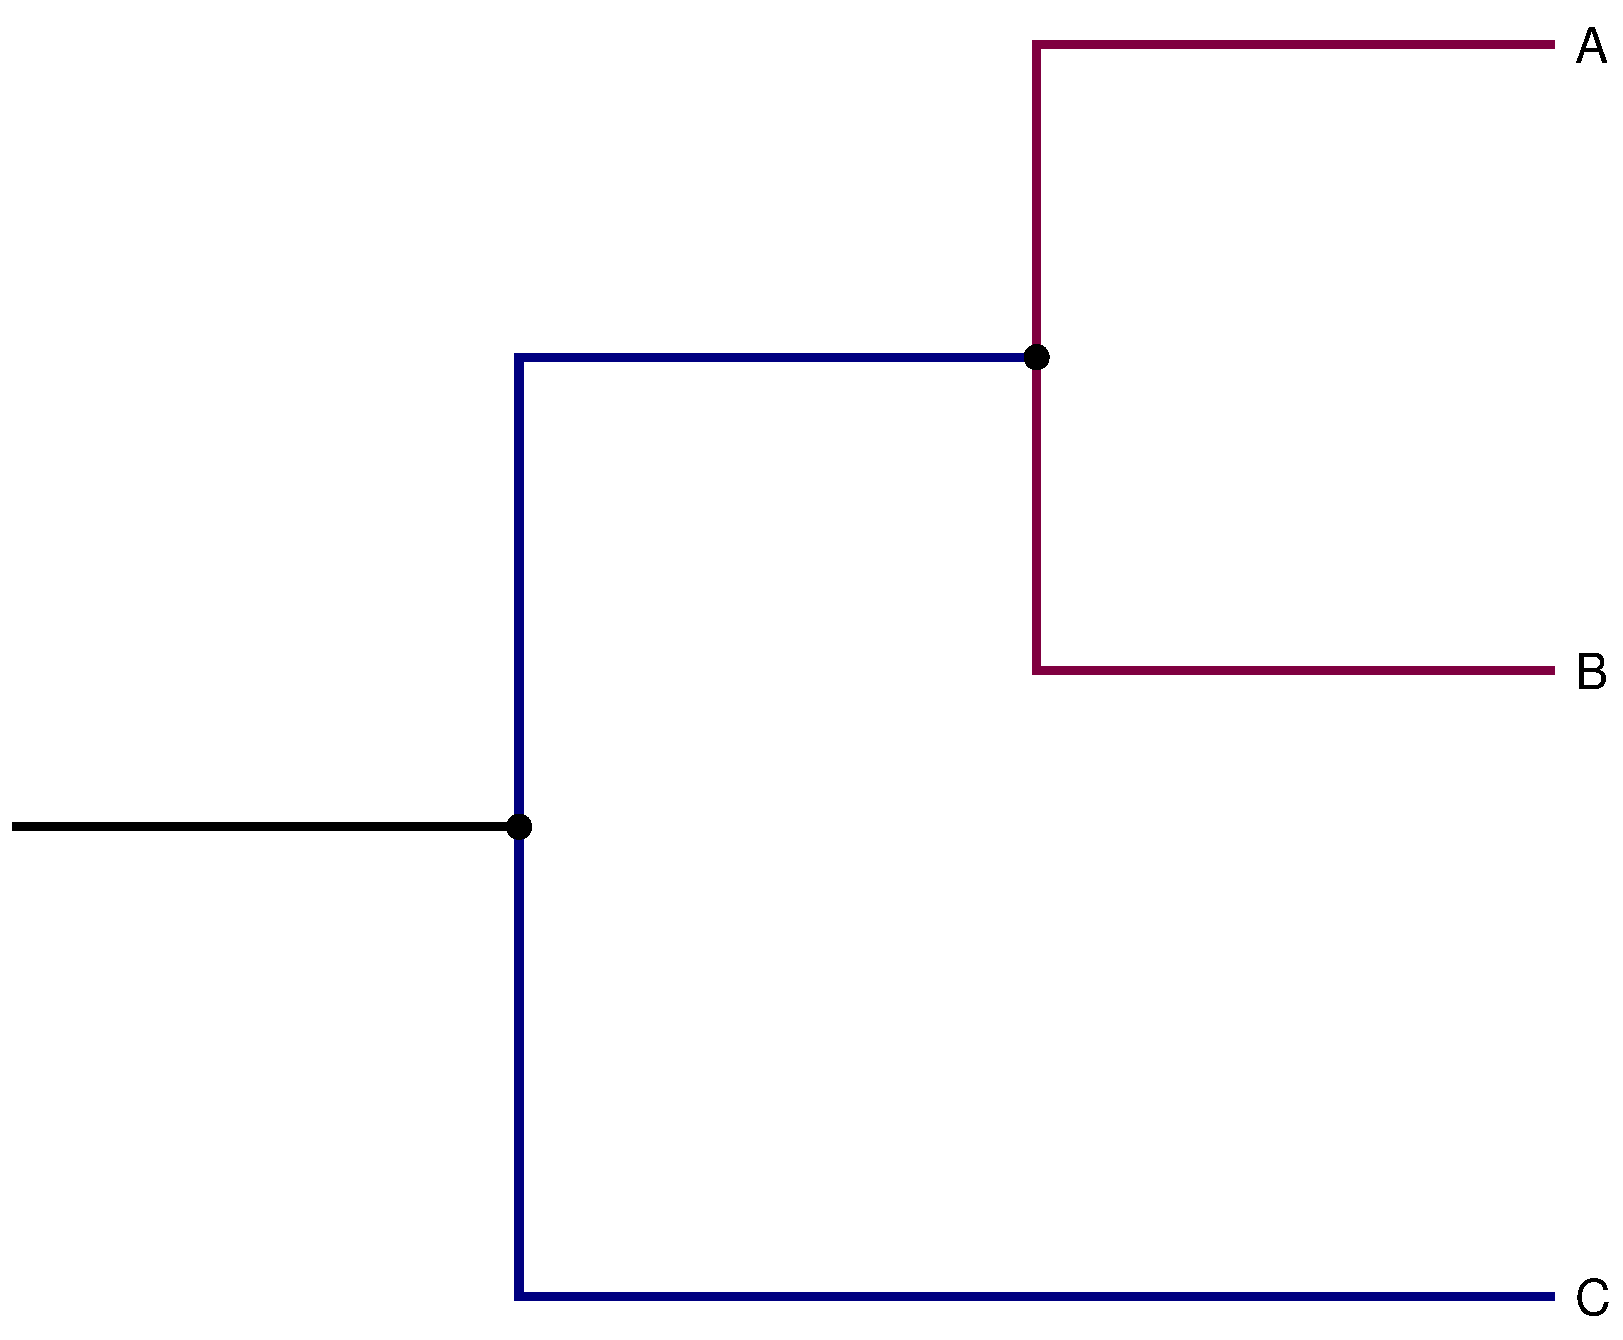
\includegraphics[width=0.33\textwidth]{./code/parallelizing_phylogeny/phylo.pdf}
     \caption{Example of phylogeny we might want to simulate. Note how branches with the same color can be simulated in parallel when there is no migration.}
     \label{fig:phylo}
    \end{figure}

In the previous section, we explored how to do a hybrid simulation, which consists of stitching together a backwards-in-time step followed by a forwards-in-time simulation.
Now, we will explore how to stitch together multiple forwards-in-time simulations, which we perform in parallel to reduce the total clock time and memory requirements.

Any two branches stemming from the same node in a species tree are independent from each other and
thus can be simulated in parallel (assuming no migration between the species).
For example, in the phylogeny depicted in Figure~\ref{fig:phylo},
branches of the same color can be simulated in parallel.
To do so, we will need to
(i) simulate the history of each branch and
(ii) join the resulting simulations together onto one multi-species history.

\subsection{Parallel simulation of branches}

First, we need to write a \slim script that will be used for simulating the history of each branch in our phylogeny.
We will perform a simple simulation,
in which each branch can have a different (but fixed) population size and length (number of ticks).
Also, we will allow deleterious mutations to happen across the entire chromosome at a fixed rate.
See the code below:

\begin{minted}[fontsize=\small, linenos, bgcolor=gray!10]{slim}
  \inputminted[breaklines, breakautoindent=true, breakanywhere=true, fontsize=\small, linenos, bgcolor=gray!10]{javascript}{./code/parallelizing_phylogeny/simulate_branch.slim}
\end{minted}

For each branch, the presence or absence of \verb|infile| tells \slim whether a previous branch exists or not.
If so, \slim will read the previous tree sequence and change the population size accordingly.
Note that when you read a tree sequence into \slim,
the tick counter will be updated with the time encoded in the tree sequence,
so we need to set the end of the simulation as the length of the branch (\verb|num_gens|)
plus the current “time” at the end of the loaded tree sequence.
At the end of the simulation, we call \verb|sim.treeSeqRememberIndividuals| right before saving the resulting tree sequence.
This is necessary because we need to ensure the individuals in the final generation are never dropped
from the tree sequence in future runs of \slim which are started from the output of the simulation,
as they will later be used to glue the tree sequences together.

The example phylogeny we will simulate is encoded in the table below (Table~\ref{tab:phylo}).

\begin{table}[h]
  \centering
  \caption{Parameters of the phylogeny that will be simulated.}
  \label{tab:phylo}
    \begin{tabular}{llll}
      \bfseries Child & \bfseries Parent & \bfseries Population size & \bfseries Edge length \\
      \hline
      \csvreader[head to column names]{./code/parallelizing_phylogeny/phylo.csv}{}%
        {\child & \parent & \popsize & \edgelen\\}
    \end{tabular}
\end{table}

There are several ways to parallelize the simulations of the branches, including a Make script, a workflow manager like Snakemake, or a breadth-first traversal of the phylogeny in Python or your favorite scripting language. For simplicity, we chose to do the parallelization in make, but see the \pyslim \href{https://tskit.dev/pyslim/docs/latest/vignette_parallel_phylo.html}{documentation} for other implementations. Note how in the Make script below, we pass parameters to the \verb|simulate_branch.slim| script to set the population size and edge length for each branch.

\inputminted[breaklines,fontsize=\small, breakanywhere=true, breakautoindent=true, linenos, bgcolor=gray!10]{basemake}{./code/parallelizing_phylogeny/parallel_sims.make}


\subsection{Putting it all together: unioning the tree sequences}

With the tree sequences in hand, we now need to glue them together.
This can be done using the \verb|union| operation from \tskit.
For two tree sequences which share some of its past history, 
union works by copying the non-shared parts of one of the tree sequence onto the other.
See Figure~\ref{fig:union} for an example of how union works.

\begin{figure}[h!]
    \centering
     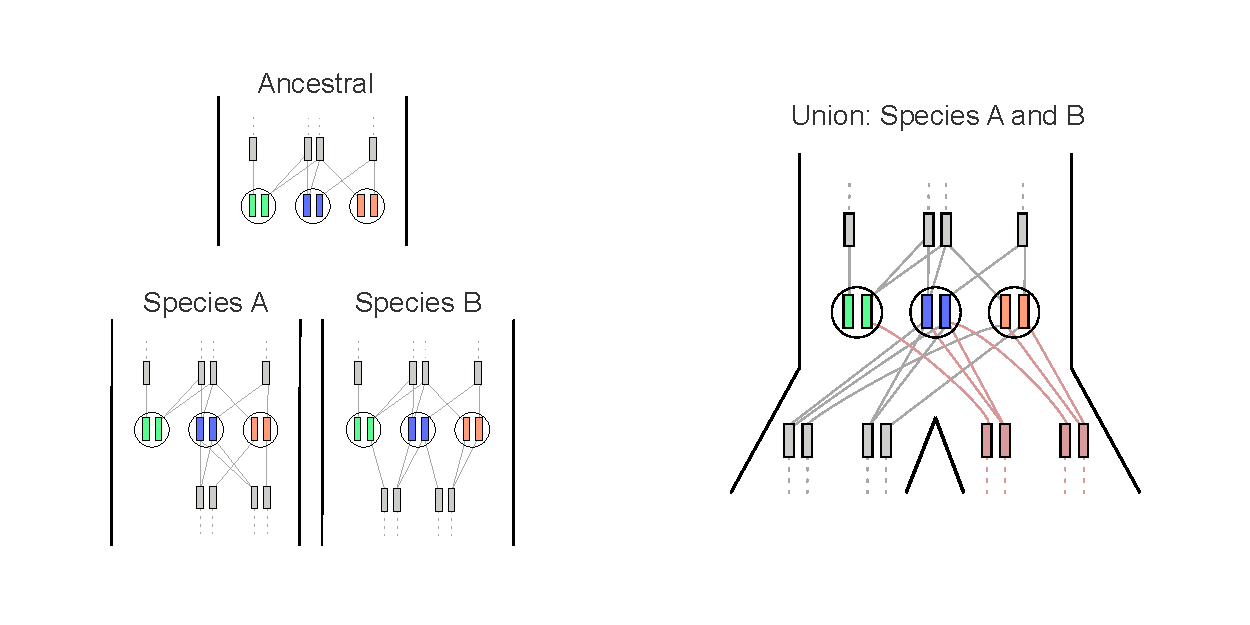
\includegraphics[width=\textwidth]{./figures/union.pdf}
     \caption{Species A and B share the same ancestral history, but after the split they are simulated independently. Note how the history above the split (delimited by the individuals which are remembered and persistent across tree sequences, highlighted in green, blue and orange) is identical. The \tskit union operation will merge these tree sequences given a map relating the nodes in the two tree sequences that are the same. In this example, union would work by adding all the history of species B that is not already present in the history of species A (nodes and edges added are highlighted in light red).}
     \label{fig:union}
    \end{figure}

The trickiest part of this operation is defining the parts that are equivalent in the two tree sequences.
For that, we will have to create an array that serves as a map of node IDs between the two tree sequences.
Below is a function that will construct a map of the node IDs of two SLiM tree sequences that correspond to the same chromosomes in SLiM at any time older than the given time ago at which the two populations split. 
Given two tree sequences \verb|other| and \verb|ts|, the goal here is to find, for each node born before \verb|split_time| ago in other, the matching node in \verb|ts|, where we can identify matching using the SLiM ID in metadata.
The code could be made easier to read by iterating over nodes, 
but the following numpy-based version is much faster.

\begin{minted}[fontsize=\small, linenos, bgcolor=gray!10]{python}
def match_nodes(other, ts, split_time):
    """
    Given SLiM tree sequences `other` and `ts`, builds a numpy array with length
    `other.num_nodes` in which the indexes represent the node id in `other` and the
    entries represent the equivalent node id in `ts`. If a node in `other` has no
    equivalent in `ts`, then the entry takes the value `tskit.NULL` (-1). The
    matching is done by comparing the IDs assigned by SLiM which are kept in
    node metadata. This matching of SLiM IDs is *only* done for nodes with time
    older than the specified `split_time`.
    """
    node_mapping = np.full(other.num_nodes, tskit.NULL)
    sids0 = np.array([n.metadata["slim_id"] for n in ts.nodes()])
    sids1 = np.array([n.metadata["slim_id"] for n in other.nodes()])
    alive_before_split1 = (other.tables.nodes.time >= split_time)
    is_1in0 = np.isin(sids1, sids0)
    both = np.logical_and(alive_before_split1, is_1in0)
    sorted_ids0 = np.argsort(sids0)
    matches = np.searchsorted(
        sids0,
        sids1[both],
        side='left',
        sorter=sorted_ids0
    )
    node_mapping[both] = sorted_ids0[matches]
    return node_mapping
\end{minted}

Now we are finally ready to union our tree sequences.
For that, I wrote a recursive function that goes through a data frame with the phylogeny
and returns a dictionary with the merged tree sequences from the tip to the root.
We could manually specify the order of unioning, but this is more flexible and general.

\begin{minted}[fontsize=\small, linenos, bgcolor=gray!10]{python}
merged = {
    row.child : {
        "ts": tskit.load(row.outfile),
        "depth": row.edgelen,
        "children": [row.child]
    }
    for i, row in df[df.is_leaf].iterrows()
}

def union_children(parent, df, merged):
    print(f"Going in: {parent}")
    child_rows = df[df.parent == parent]
    assert (len(child_rows) == 2) or (len(childs) == 0)
    if len(child_rows) == 2:
        children = [row.child for _, row in child_rows.iterrows()]
        for child in children:
            if child not in merged:
                union_children(child, df, merged)
        split_time = merged[children[0]]["depth"]
        assert split_time == merged[children[1]]["depth"] # ultrametric
        print(f'Unioning: {children}, Split time: {split_time}')
        ts0 = merged[children[0]]["ts"]
        ts1 = merged[children[1]]["ts"]
        node_map = match_nodes(ts1, ts0, split_time)
        tsu = ts0.union(ts1, node_map, check_shared_equality=True)
        # the time from tip to start of simulation is split_time plus the
        # length of the edge
        parent_edgelength = df[df.child==parent].edgelen.item()
        merged[parent] = {
            "ts": tsu,
            "depth": split_time + parent_edgelength,
            "children": merged[children[0]]["children"] + merged[children[1]]["children"]
        }

union_children("root", df, merged)
# union of all three species tree sequences is in the root.
tsu = merged["root"]["ts"]
pops = merged["root"]["children"]
\end{minted}

We had keep track of which population in the union’ed tree sequence corresponds to which population in our phylogeny.
Happily, we’ve stored each population’s name in its metadata field, 
so it’s easy to match populations in the tree sequence up to what they’re supposed to be.
Now, we have a union'ed tree sequence of the entire phylogeny we depicted in Figure~\ref{fig:phylo},
which we can use for our downstream analyses.

In this section, we learned how to parallelize forward-in-time simulations of multiple species.
The biggest upside of this strategy is that it allows us to simulate a large number of species,
which wouldn't be possible within a single simulation due to memory constraints.
For example, in \citet{rodrigues2024shared} it was possible to dom whole-chromosome simulations of the entire great apes history,
spanning over 10 million years, using a similar approach to the one presented here.
Even though the memory burden of the simulation was distributed across multiple processes,
single-species simulations would still used over 100Gb of memory.
Thus, simulating all the great apes species in a single process would have been impossible.


%%%%%%%%%%%%%%%%%%%%%%%%%
\section*{Modelling meta-population dynamics with simulation networks}

Our final vignette will explore two extensions of the previous section on parallelizing \slim simulations in the context of
a model of pathogen evolution.
Let us imagine a pathogen that infects a host population, such as humans. We can model the pathogen as
a large metapopulation, where each infected human host constitutes a distinct deme, and whose evolutionary
dynamics are significantly shaped by the interactions among the hosts. We will take advantage of parallelization
to reduce the computational burden of realistically representing the size and structure
of a pathogen population as well as the among-host and within-host dynamics.

Similar to our phylogeny in the previous section, we can represent the relationship between individual hosts
with a simple branching structure. In this figure, host individuals are represented by nodes and transmissions
from one host to another are represented by edges.
Within this branching tree structure, each host infection (or node) is modeled by a separate instance of a
SLiM model that represents the pathogens infecting and replicating in that host (see full model on github).

%% insert code block
%%

This model has a simple but flexible structure that loads in an input tree sequence, simulates the exponential growth of
pathogen individuals within the host, and then simulates a strong population bottleneck as the pathogen is then
transmitted on to the next host. These dynamics will play out repeatedly as the pathogen spreads through the host population.

This framework makes it feasible to represent an extremely large pathogen (census) population size, but it also
creates in some unique challenges. First, we have to figure out how to stitch together the multiple tree sequences
that will result from this process by coming up with a way to identify shared subsets of multiple tree sequences.

Next, we 

%%% SSG STOPPED 7/9



Let us also imagine that there exists a genetic variant in the pathogen population that underlies a life history trade-off between replication and transmissibility; one allele allows the individual carrying it to reproduce at a faster rate while the alternate allele increases an individual’s likelihood of being transmitted to a new host. This kind of trade-off has been observed in influenza, HIV, and COVID-19 [cite], so this kind of model could shed light on the evolutionary dynamics of these viruses…
As previously discussed, we can generate initial neutral diversity for our model by either conducting a burn-in or recapitation. 

Pathogens often have very large population (census) sizes,
but spread out across many host individuals with between-host dynamics
that are daunting to simulate.
However, the dynamics \emph{within} a host are closer to a standard \slim simulation,
which makes this a good target for parallelization:
the dynamics within each host is a single job;
each job may create new jobs (new infections)
or interact with other jobs (co-infection).
Maintaining a tree sequence across these runs is conceptually similar
to the previous section, but has additional difficulties.

To do this, we have a \slim script that describes dynamics within a single host.
This script begins by loading in a tree sequence
that contains the pathogen individual(s) that initiated the infection and their history,
and at some later point writes out a tree sequence containing the individual(s) that infect other host(s)
and their history.
Then, we use job scheduling software to organize the simulation runs.
There are thus two important steps to describe:
first, how individuals are ``transmitted'' from one simulation to the next;
and second, how we combine the resulting tree sequences.
There are various ways to set this up; we describe one method that makes bookkeeping
less daunting.

A first attempt at transmission between hosts would simply save the state of the population
at the desired time, and then the \slim run describing the next host
would start from this state by selecting a few individuals as those that were transmitted.
However, this can easily lead to contradictions: for instance,
if one host infects two other hosts,
then a single individual who was present in the first host simulation
might die at different times in the simulation runs of the two subsequent hosts.
So, coordination is required.
\slim can write out arbitrary information to text files,
but the most convenient place to record auxilliary information that goes along with a given tree sequence
is usually in the ``top-level metadata'',
which is visible in both \slim and python as a dictionary
(in python, as \verb|ts.metadata|).
So, whenever a new host is to be infected,
we select some ``founder'' individuals to start the infection;
Remember these founders and then kill them;
and then write down their IDs in the metadata
(under a key which identifies the host they're going on to infect).
Then for each subsequent host
we use a python script to post-process the resulting tree sequence
so that the founder individuals will be ``alive'' (and no others)
when the tree sequence is loaded into \slim.

The next task is to combine the partially-overlapping histories of different hosts.
As in the previous section, we use \verb|union| to do this;
however, we need to work a little harder
to identify the portions of history that are shared between two tree sequences.
To do this, we need to
(a) find the founders that are present in both tree sequences,
and (b) identify all nodes that are ancestral to these founders.
The first step is easily done by consulting metadata.
Here is code that identifies all ancestors in the tree sequence
of a given set of nodes:
\comment{Either remove this; move it to the appendix; or explain what it's doing.}
\begin{minted}[fontsize=\small, linenos, bgcolor=gray!10]{python}
def ancestors(ts, nodes):
    """
    Returns the list of nodes reachable from `nodes` by following
    child->parent relationships in the edge table.
    """
    out = np.zeros(ts.num_nodes, dtype='int')
    out[nodes] = 1
    x = out.copy()
    A = scipy.sparse.coo_array(
            (
                np.ones(ts.num_edges, dtype='int'),
                (ts.edges_parent, ts.edges_child)
            ), dtype='int', shape=(ts.num_nodes, ts.num_nodes)
    )
    while np.sum(x) > 0:
        x = A @ x
        out += x
    return np.where(out > 0)[0]
\end{minted}
With this in hand, we can use \verb|union|
as in the prvious section.


%%%%%%%%%%%%%%%%%%%%%%%%%
\section*{Discussion}

The use of ARGs in simulation is powerful,
since a great deal more information can be recorded about the simulation
while making the simulation more efficient as well \citep{kelleher2016efficient}.
The ARG can be used to exchange information between simulators as well.
The most commonly useful example of this is perhaps \emph{recapitation},
which allows the prior history of a forwards-time simulation
to be simulated \emph{post hoc} with a coalescent simulator.
However, nuances of exactly which ancestors and what portions of history
are stored in a given ARG can be tricky.
In this chapter, we've aimed to introduce the reader to the topic,
to several useful tools from \pyslim,
and to present several useful techniques.

An important matter we have not covered in detail here is \emph{time units}.
First, ``time'' in \slim goes forwards, while ``time'' as recorded in the tree sequence goes backwards (i.e., it is ``time ago'').
In matching these up correctly there are myriad possibilities for off-by-one errors.
More importantly, in \slim's non-Wright-Fisher models one time unit may not equal one generation,
and so adjustment to the time units used by \msprime is necessary.
Both these cases are covered in more detail in the \pyslim documentation.

A general theme here (and in simulation work generally)
is a tradeoff between realism and efficiency.
Since forwards-time simulations more naturally match real population dynamics,
it would for most cases be conceptually simpler to implement a single \slim simulation.
However, many situations we'd like to study lead to computationally intractable simulations,
and so coalescent simulation becomes useful or even necessary.
The same trade-off occurs when considering rescaling \citep{cury_simulation_2022,dabi_population_2025}.
A general principle to remember in these cases is that a coalescent simulation is equivalent
to simulation from a certain neutral model of discrete populations.
If there are concerns about the validity of the approximation,
then a good strategy is to adjust the parameters of the approximation (e.g., how long ago recapitation is applied)
and see if important conclusions are affected.


%%%%%%%%%%%%%%%%%%%%%%%%%
\section*{Author contributions}


\bibliographystyle{plainnat}
\bibliography{./references.bib} % Looks for mybib/references.bib

%%%%%%%%%%%%%%
\newpage
\appendix

\comment{STUFF WE MAYBE DON'T WANT: moved here from above:}

\comment{Remove ILS thing and just add a paragraph citing Rodrigues et al and saying why this would be faster and would split the memory requirements across a bunch of processes.}

\section{Recapitation}


Doing this is as simple as:

\begin{minted}[fontsize=\small, linenos, bgcolor=gray!10]{slim}
orig_ts = tskit.load("example_sim.trees")
rts = pyslim.recapitate(orig_ts,
            recombination_rate=1e-8,
            ancestral_Ne=200, random_seed=5)
\end{minted}
The warning is harmless; it is reminding us to think about generation time
when recapitating a nonWF simulation (a topic we'll deal with later).

We can check that this worked as expected, by verifying that after recapitation
all trees have only one root:
\begin{minted}[fontsize=\small, linenos, bgcolor=gray!10]{slim}
orig_max_roots = max(t.num_roots for t in orig_ts.trees())
recap_max_roots = max(t.num_roots for t in rts.trees())
print(f"Maximum number of roots before recapitation: {orig_max_roots}\n"
      f"After recapitation: {recap_max_roots}")
\end{minted}

The `.recapitate` method
is just a thin wrapper around `msprime.sim\_ancestry`,
and you need to set up demography explicitly - for instance, in the example above
we've simulated from an ancestral population of ``Ne=200`` diploids.
If you have more than one population,
you must set migration rates or else coalescence will never happen.
% (see [](sec_recapitate_with_migration) for an example, and {func}`.recapitate` for more).

(TODO: mention about how to recapitate with a nonuniform map, as in the docs?)


\section{Simplification}


Probably, your simulations have produced many more fictitious genomes
than you will be lucky enough to have in real life,
so at some point you may want to reduce your dataset to a realistic sample size.
We can get rid of unneeded samples and any extra information from them by using
an operation called *simplification* (this is the same basic approach that SLiM
implements under the hood when outputting a tree sequence).

Depicted in Figure~\ref{fig:recap_simp}B is the result of applying an explicit call to
simplify to our example tree sequence.
In the call we asked to keep only 4
genomes (contained in 2 of the individuals in the current generation). This has
substantially simplified the tree sequence, because only information relevant to the
genealogies of the 4 sample nodes has been kept. (Precisely, simplification retains only
nodes of the tree sequence that are branching points of some marginal genealogy -- see
CITE % [Kelleher et al 2018](https://doi.org/10.1371/journal.pcbi.1006581) for details.)
While simplification sounds very appealing - it makes things simpler after all -
it is often not necessary in practice, because tree sequences are very compact,
and many operations with them are quite fast.
(It will, however, speed up many operations, so if you plan to do a large number of simulations,
your workflow could benefit from early simplification.)
So, you should probably not make simplification a standard step in your workflow,
only using it if necessary.

It is important that simplification - if it happens at all -
either (a) comes after recapitation, or (b) is done with the
``keep\_input\_roots=True`` option.
This is because simplification removes some of the
ancestral genomes in the first generation,
which are necessary for recapitation,
unless it is asked to "keep the input roots".
If we simplify without this option before recapitating,
some of the first-generation blue chromosomes in the figure on the right
would not be present, so the coalescent simulation would start from a more recent point in time
than it really should.
As an extreme example, suppose our SLiM simulation has a single diploid who has reproduced
by clonal reproduction for 1,000 generations,
so that the final tree sequence is just two vertical lines of descent going back
to the two chromosomes in the initial individual alive 1,000 generations ago.
Recapitation would produce a shared history for these two chromosomes,
that would coalesce some time longer ago than 1,000 generations.
However, if we simplified first, then those two branches going back 1,000 generations would be removed,
since they don't convey any information about the shape of the tree;
and so recapitation might produce a common ancestor more recently than 1,000 generations,
which would be inconsistent with the SLiM simulation.

After recapitation,
simplification to the history of 100 individuals alive today
can be done with the {meth}`tskit.TreeSequence.simplify` method:
\begin{minted}[fontsize=\small, linenos, bgcolor=gray!10]{slim}
import numpy as np
rng = np.random.default_rng(seed=3)
alive_inds = pyslim.individuals_alive_at(rts, 0)
keep_indivs = rng.choice(alive_inds, 100, replace=False)
keep_nodes = []
for i in keep_indivs:
  keep_nodes.extend(rts.individual(i).nodes)

sts = rts.simplify(keep_nodes, keep_input_roots=True)
\end{minted}

Note that you must pass simplify a list of \textit{node IDs}, not individual IDs.
Here, we used the `.individuals\_alive\_at` method to obtain the list
of individuals alive today.
Also note that there are *still* more than 100 individuals remaining - 15 non-sample individuals
have not been simplified away,
because they have nodes that are required to describe the genealogies of the samples.
(Since this is a non-Wright-Fisher simulation,
parents and children can be both alive at the same time in the final generation.)



\section{Adding neutral mutations to a SLiM simulation}

% ```{figure} _static/pedigree_mutate.png

If you have recorded a tree sequence in SLiM, likely you have not included any neutral mutations,
since it is much more efficient to simply add these on afterwards.
To add these (in a completely equivalent way to having included them during the simulation),
you can use the `msprime.sim\_mutations` function, which returns a new tree sequence with additional mutations.
Continuing with the cartoons from above, these are added to each branch of the tree sequence
at the rate per unit time that you request.
We'll add these using the {class}`msprime.SLiMMutationModel`, so that the file can be read back into SLiM,
but any of the other mutation models in msprime could be used.
This works as follows:
\begin{minted}[fontsize=\small, linenos, bgcolor=gray!10]{slim}
next_id = pyslim.next_slim_mutation_id(sts)
ts = msprime.sim_mutations(
           sts,
           rate=1e-8,
           model=msprime.SLiMMutationModel(type=0, next_id=next_id),
           keep=True,
)
\end{minted}


What's going on here? Let's step through the code.

\begin{enumerate}
    \item The mutation ``rate = 1e-8``, which adds mutations at a rate of $10^{-8}$ per bp.
    Unlike previous versions of msprime, this adds mutations using a discrete-sites model,
    i.e., only at integer locations (like SLiM).

\item We're passing ``type=0`` to the mutation model.
    This is because SLiM mutations need a "mutation type",
    and it makes the most sense if we add a type that was unused in the simulation.
    In this example we don't have any existing mutation types, so we can safely use ``type=0``.

\item We also add ``keep = True``, to keep any existing mutations.
    In this example there aren't any, so this isn't strictly necessary,
    but this is a good default.

\item If there are existing SLiM mutations on the tree sequence we need to
    make sure any newly added mutations have distinct SLiM IDs,
    so we use `.next\_slim\_mutation\_id` to figure out
    what the next available ID is, and pass it in.

\end{enumerate}

TODO: writing out to VCF



\end{document}
